\documentclass[12pt, dvipdfmx]{jarticle}
\usepackage{ilsfonts}    % 卒論スタイルで使うフォントの定義
\usepackage{ilssoturon}  % 卒論スタイル宣言
\usepackage[dvips]{graphicx} % グラフィクスの利用宣言
\usepackage{amsmath,amssymb} % 数学記号などの利用宣言
\usepackage{bm}  % 太字数式文字の利用に関する宣言
%\usepackage{slashbox} % 表に斜線を入れる(不要かも)
%\usepackage[dvips]{graphicx,psfrag} % 図に数式を使うときに用いる(別の方法がおすすめ)
\usepackage[dvipdfmx]{graphicx} %図
% ハイパーリンクを作るためのパッケージだが,pdf viewerによってはハイパーリンクの枠が描画されたまま出力されるので,基本的には使用しない
%\usepackage[dvipdfmx]{hyperref}
%\usepackage{pxjahyper} % 日本語しおりを作るためのパッケージ

\年度{2023年度} % 以下は論文表紙に出力される内容
\提出日{2024年1月xx日}
\研究者{2031133 &増田 瑞樹}
\論文題目{WANNにおける活性化関数の慎重な選択}

\begin{document} % ここから論文本体
\卒論表紙 % これで数式が出る

% 正しく目次を出力するためには tex コンパイルを2回連続でかけること
\pagenumbering{roman} % 目次のページ番号はローマ数字

\tableofcontents % 目次を出す命令
\clearpage % 改ページ

\pagenumbering{arabic} % ページ番号をアラビア数字になおす

\section{はじめに}
生物学における先天的能力(Precociality)とは,動物が生まれた瞬間からすでに持っている能力のことである.例えば,トカゲやヘビは生まれ持って捕食者から逃れる能力を有している.また,アヒルは孵化後すぐに泳いだり食事をすることができ,七面鳥は一度も見たことがない捕食者を視認するすることができる.これは,動物の脳は高度に構造化された状態で生まれ,その構造はゲノムに記憶されていることを意味する.Zadorは生物学的な学習について『動物の行動の多くは生得的なものであり学習によって生じるものではない.動物の脳はAI研究者が思い描くようななんでも学べる汎用的な学習アルゴリズムを備えた白紙の状態ではない.』と強調している\cite{先天的能力}.\\
Weight Agnostic Neural Networks(WANN)は,2019年にAdam GaierとDavid Haによって発表されたシナプス荷重に依存しないネットワークの探索アルゴリズムである\cite{WANN}.WANNは,NEAT\cite{NEAT}をベースに作られており,どのようなシナプス荷重においてもタスクを解ける性質をもつネットワーク,つまり構造自体にタスクを解く機能が備わっている.これは遺伝的アルゴリズム\cite{遺伝的アルゴリズム}を用いたNeuro-Evolution\cite{NE}の手法から実現できる.\\
WANNの個体変異の1つに,ノードの活性化関数の変更が行われる.隠れ層からランダムに選択されたノードの活性化関数は現在採用されている以外の活性化関数に同様に確からしく選択される.これは探索後期において,それまでの良かったノードの出力を反転させてしまう懸念がある.\\
本論文では,活性化関数を変更する際の確率を関数同士の距離関数が小さいほど選ばれやすいようにする手法を提案する.距離関数が小さいことは,関数同士が似ているを意味し,活性化関数の変更により出力の大きな変更が起こりにくくなる.距離関数には0付近の活性化関数同士の出力の差を積分と,実際にその個体が体験した入力ノードから推測できる該当ノードの出力の差の合計を採用する.\\
実験では \textbf{ここから追加} %はじめに
\clearpage

\section{ニューラルネットワーク}
\subsection{ニューラル素子}
人間を含む生命の脳を構成する神経細胞はニューロンと呼ばれ,人間の脳には140億個のニューロンがありそれぞれのニューロンは平均約8,000個のシナプスを持つとされている.ニューラルネットワークのノードはニューロンをモデルとし,計算機上でニューロンをシミュレートできるよう設計されている.
\\ \textbf{ここに図} \\
ここでは,素子への $ N $ 個の入力 $ S_1, S_2, ..., S_N $ に対して各々の重み $ w_1, w_2, ..., w_N $ となっている.この素子は入力からバイアス $ b $ を足した値を活性化関数 $ f $ の入力とし,活性化関数の出力をノードの出力 $ z $ とする.

\begin{equation}
    z = f(\sum_{i=1}^N S_i + b)
\end{equation}

主に活性化関数 $ f $ には次のような関数を用いる.

\begin{enumerate}
    \item tanh関数
    \begin{equation}
        f(x) = \frac{e^{x} - e^{-x}}{e^{x} + e^{-x}}
    \end{equation}

    \item ReLU関数
    \begin{equation}
        f(x) = 
        \begin{cases}
        x & (x > 0)\\
        0 & (x \leq 0)
        \end{cases}
    \end{equation}
\end{enumerate} %ニューラルネットワーク
\clearpage

\section{遺伝的アルゴリズム}
遺伝的アルゴリズム(GA)とは,適用範囲の非常に広い,生物の進化を模倣した学習的アルゴリズムである\cite{遺伝的アルゴリズム}.すなわち何万年,何億年もかけて生物の特徴が進化してきたような遺伝的法則を光学的な手法にモデル化し,また参考にしてタスクを解くものである.自然界における生物の進化過程においては,ある世代を形成している個体の集合,すなわち個体群の中で環境に適している個体が高い確率で生き残り,生き残った個体は交叉や突然変異によって次の世代の個体群が形成される.

\subsection{本論文における基本的動作}
本論文において,新しく個体を形成する際に交叉は使用しない.以降本論文で用いる遺伝的アルゴリズム変則GAと呼ぶ.図は変則GAの動作を流れを表している.

\begin{figure}[h]
    \begin{center}
        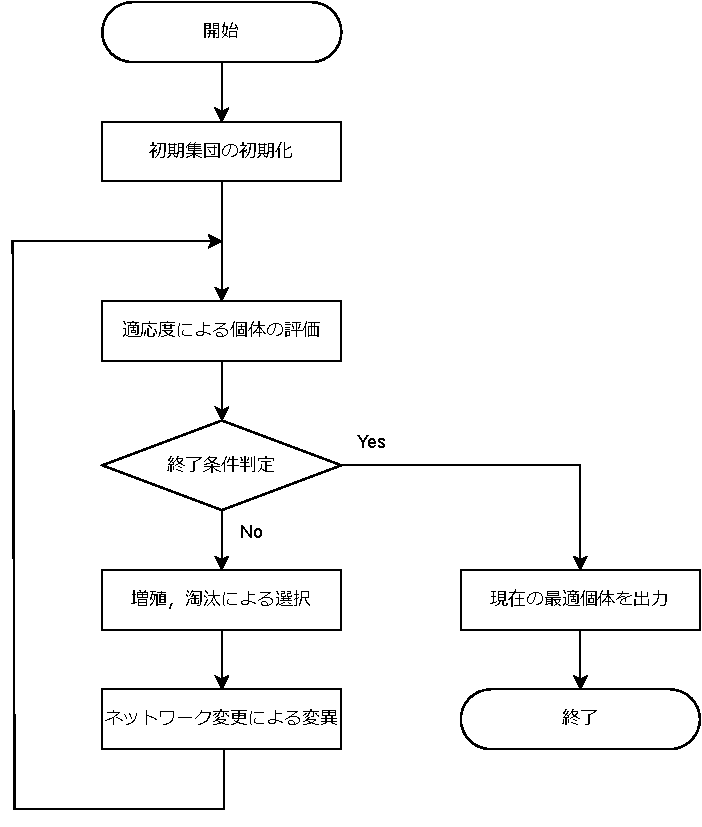
\includegraphics[scale=0.8]{img/expga.pdf}
        \caption{変則GAの概要}
    \end{center}
\end{figure}


\begin{enumerate}
    \item 初期化 \\
    ランダムな性質を持つ個体を $ N $ 個生成し,初期世代の個体群を設定する.

    \item 評価 \\
    各個体についてタスクを解かせ,その進捗により適応度を測定する.

    \item 終了判定 \\
    終了条件を満たしていれば,その時に得られる最適個体を問題の準最適解として出力する.

    \item 選択 \\
    各個体に対応する適応度により並べ替え,適応度の低い個体は淘汰され,適応度の高い個体は増殖する.

    \item 変異 \\
    設定された突然変異の設定により変異を行い,新しい個体群を生成する.変異を行った後の個体群は次世代の個体群として再度評価される.
\end{enumerate}

終了判定には最良個体の適応度や個体群の平均の適応度を参照する場合が多いが,本論文ではあらかじめ設定した世代数を超えたときにのみ終了判定が真になり,プログラムは終了する.また,変異をする過程でエリート保存選択を実行する.これは非常に優れた個体は変異をする前の状態のほうが変異をした後の状態よりも優れている見込みが大きいことから,個体に対して変異を行わず,全く同じ状態の個体を次世代に残す手法である.エリート保存選択は,むやみに変異をして優良個体の遺伝子を破壊しないことにつながる.

\subsection{ルーレット選択}
ルーレット選択は,個体群の中の各個体の適応度とその総計を求めて,適応度の総計に対する各個体の割合を選択確率として個体を選択するという基本的な考えに基づいている\cite{遺伝的アルゴリズム}.すなわち,ルーレット選択では,個体 $ s_i $ の適応度 $ f{s_i} $ と個体群の総計を求め,個体 $ s_i $ が選択される確率を

\begin{equation}
    P_i = \frac{f(s_i)}{\sum^N_{j=1} f(s_j)}
\end{equation}

として個体の確率的に選択する.このようなルーレット選択のアルゴリズムは,次のように要約される.

\begin{enumerate}
    \item 世代 $ t $ の個体群 $ X(t) $ の中の $ N $ 個の個体の適応度 $ f_i $ とその総計 $ f_{sum} = \sum^N_{i=1} f_i $ を求める.

    \item 区間[0, 1]の乱数 $ rand $ を発生させ, $ s = rand \times f_{sum} $ とする.

    \item $ \sum^k_{i=1} f_i \geq s $ となるような最小の $ k $ を求めて, $ k $ 番目の個体を世代 $ t+1 $ に生き残る個体の候補とする.

    \item 候補となる個体数が $ N $ になるまで2, 3を繰り返す.
\end{enumerate}

本論文ではルーレット選択を個体の変異先を選択する際に用いる.同じ構造を持つネットワークの,ひとつのノードの活性化関数のみを変更し,この出力が小さいほど $ f_i $ が大きいことになる.
 %遺伝的アルゴリズム
\clearpage

\section{神経科学}
\subsection{サブタイトル}
内容
 %神経科学
\clearpage

\section{Weight Agnostic Neural Networks}

\begin{figure}[h]
    \begin{center}
        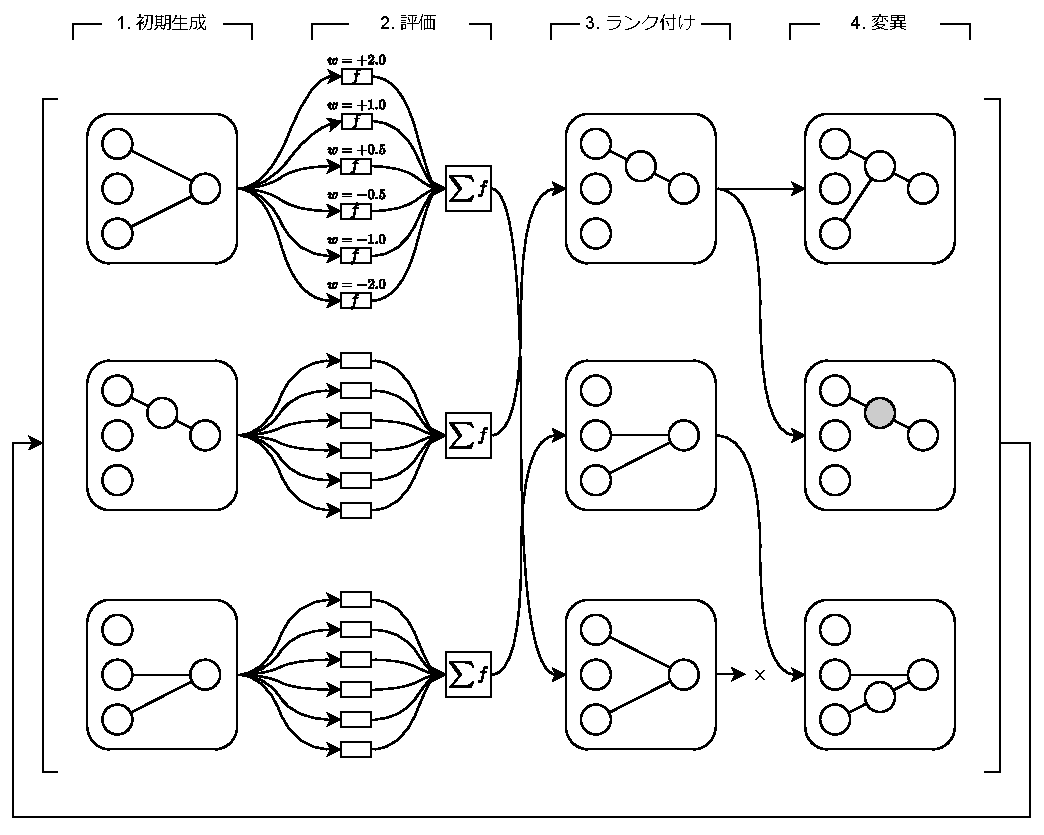
\includegraphics[scale=0.8]{img/expwann.pdf}
        \caption{WANNsの概略図}
    \end{center}
\end{figure}

Weight Agnostic Neural Networks(WANNs)は,2019年にAdam GaierとDavid Haによって発表されたニューラルネットワークの構造探索アルゴリズムである\cite{WANN}.WANNは,NEAT\cite{NEAT}をベースに作られており,これは遺伝的アルゴリズム\cite{遺伝的アルゴリズム}を用いたNeuro-Evolution\cite{NE}の手法から実現できる.多くのニューラルネットワークはシナプス荷重を更新することで,ネットワークの精度を向上させているが,WANNsによって生成された個体は,ネットワーク構造自体がタスクを解く性質を持っており,どんなシナプス荷重においてもそれなりの精度でタスクを解くことができる.これは生物の先天的能力と似た性質であると言える\cite{先天的能力}.また,WANNsネットワークはそれぞれのノードが別々の活性化関数を持っている.WANNの概略図を図3に示す.WANNにおける探索は以下の動作によって実現する.

\begin{enumerate}
    \item 初期生成
    個体は最初,最もシンプルな構造を持つネットワークからなる.中間層は存在せず,入力層のうちの一部からシナプスが出力層に接続されている.

    \item 評価
    各個体に対して,ネットワーク全体の共有重みを使用してタスクを実行する.本論文では, $ -2.0, -1.0, -0.5, +0.5, +1.0, +2.0 $ の6つの共有重みを使用する.また,タスクを解く際の初期状態により優れた結果を残せずに誤った評価をしないよう,それぞれの共有重みにて4回のタスクを実行する.最終的に6つの共有重みと4回の試行から得られた24個の評価値を合計する.

    \item ランク付け
    個体をランク付けする.上位の優れた個体は変更のないまま次世代へ保存され,下位の劣った個体は淘汰される.このランク付けはネットワークの評価値とネットワークの複雑さから算出される.

    \item 変異
    個体をランクのトーナメント選択\cite{遺伝的アルゴリズム}によって選択し,変異を起こした次世代の個体として保存する.

    保存された個体は再度評価,ランク付け,変異を行い,任意の世代数まで繰り返される.
\end{enumerate}

ニューラルネットワークには,その用途を達成するために適したネットワーク構造がある.画像認識には畳み込みニューラルネットワーク(CNN),自然言語処理には再起型ニューラルネットワーク(RNN)などを用いることで全結合型ニューラルネットワークよりも少ない計算量でよりよい精度を実現することができる\cite{深層学習}.自然界においても海には魚類,陸上には哺乳類などある環境下に適した身体的特徴や先天的能力をさまざまな生物が獲得している\cite{先天的能力}.ラットは生まれてから経験したことを,少なくとも小脳皮質のシナプスを追加することによってよりよいフィードバックができるように学習する\cite{シナプス学習}.WANNsはあるタスクにおいてのみ優れた精度を持つニューラルネットワークを探索するアルゴリズムで,今までのネットワーク構造ありきのシナプス重みを重視する手法とは違い,どんな重みであっても動作するネットワーク構造に着目した手法であり,生物の基本的な性質を踏襲したものになっている.結果として,十分に世代を重ねたときの最良個体の出力は,0付近を除いたすべての共有重みを用いた際に安定している.
\begin{figure}[h]
    \begin{center}
        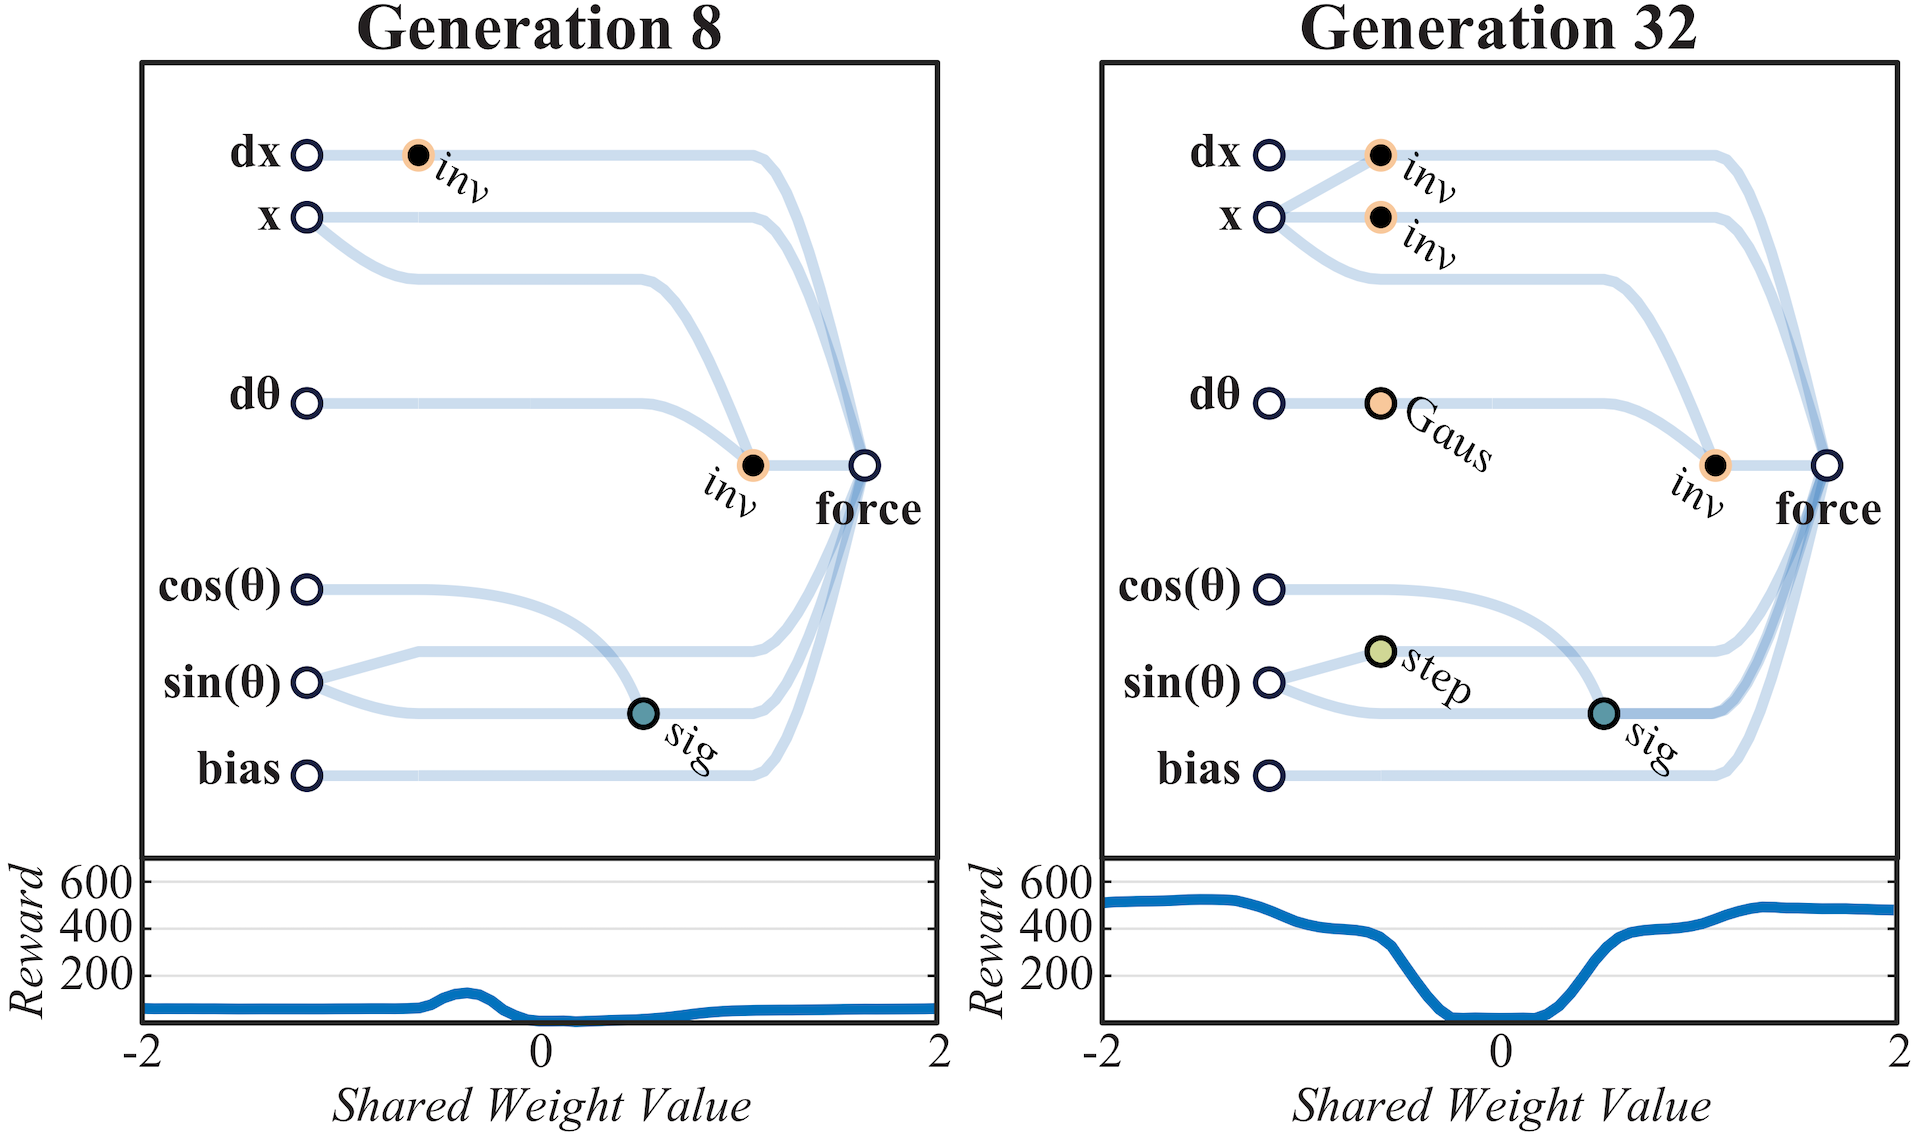
\includegraphics[width=120mm]{img/wannweight.png}
        \caption{WANNsのネットワーク構造と共有重み}
    \end{center}
\end{figure}


\subsection{変異}

\begin{figure}[h]
    \begin{center}
        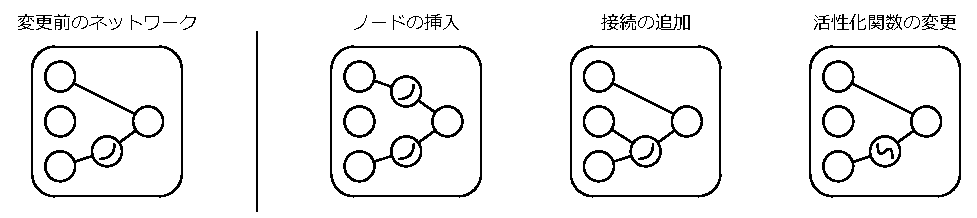
\includegraphics[scale=0.8]{img/vary.pdf}
        \caption{WANNsのネットワーク変異}
    \end{center}
\end{figure}

図に示したように,個体の変異にはノードの挿入,接続の追加,活性化関数の変更のいずれかを行い,各操作の具体的な手順は以下のようになる.

\begin{enumerate}
    \item ノードの挿入
    ネットワークの持つひとつの接続をランダムに選択し,接続の途中にひとつのノードを追加する.この時の活性化関数はランダムに選択される.

    \item 接続の追加
    接続を持たないふたつのノードを選択し,それらをつなぐ接続を追加する.

    \item 活性化関数の変更
    ネットワークの持つ中間層のノードを選択し,そのノードの活性化関数を変更する.活性化関数は現在選択されている関数以外の関数がランダムに選択される.このときの活性化関数はlinear, step, sin, cosine, Gaussian, tanh, sigmoid, inverse, absolute value, ReLUを利用する.
\end{enumerate} %WANN
\clearpage

\謝辞 % ここから謝辞
山口先生有り難う! % 謝辞のないよう
\clearpage

\begin{thebibliography}{99}
    \bibitem{WANN} \
    Gaier, Adam, and David Ha. \
    "Weight agnostic neural networks." \
    Advances in neural information processing systems 32 (2019).

    \bibitem{NEAT} \
    Stanley, Kenneth O., and Risto Miikkulainen. \
    "Evolving neural networks through augmenting topologies." \
    Evolutionary computation 10.2 (2002): 99-127.

    \bibitem{先天的能力} \
    Zador, Anthony M. \
    "A critique of pure learning and what artificial neural networks can learn from animal brains." \
    Nature communications 10.1 (2019): 3770.

    \bibitem{NE} \
    Braun, Heinrich, and Joachim Weisbrod. \
    "Evolving neural feedforward networks." \
    Artificial Neural Nets and Genetic Algorithms: Proceedings of the International Conference in Innsbruck, Austria, 1993. Vienna: Springer Vienna, 1993.

    \bibitem{遺伝的アルゴリズム} \
    坂和正敏, 田中雅博. \
    "遺伝的アルゴリズム" \
    朝倉書店 (2002).

    \bibitem{深層学習} \
    伊庭斉志. \
    "進化計算と深層学習 -創発する知能-" \
    オーム社 (2015). 

    \bibitem{活性化関数} Dubey, Shiv Ram, Satish Kumar Singh, and Bidyut Baran Chaudhuri. "Activation functions in deep learning: A comprehensive survey and benchmark." Neurocomputing (2022).
\end{thebibliography} %参考文献
\clearpage

\end{document}
